\chapter{Fundamentaci�n te�rica}\label{c:chapter1}
\section*{Introducci�n del cap�tulo}
En el presente cap�tulo se engloban aspectos relacionados con el objeto de estudio definido para el problema planteado. El an�lisis de algunas metodolog�as, procedimientos, herramientas existentes para el desarrollo de sistemas web y el an�lisis de aplicaciones hom�logas; permitir� la selecci�n de las tecnolog�as adecuadas para el desarrollo del \cdis\ y contar con un an�lisis de sistemas existentes que realizan funcionalidades similares.

\section{Proceso de comisi�n disciplinaria en la Facultad 4}\label{process}
%TODO
%Descripci�n del proceso de comisi�n disciplinaria en la Facultad 4
El proceso de comisi�n disciplinaria comienza cuando un profesor o estudiante de la \uci presenta una denuncia ante el Decano de la Facultad. El Decano de la Facultad es el encargado de verificar la veracidad de la denuncia y de asignar una comisi�n disciplinaria para que investigue el caso. Esta es la encargada de realizar la investigaci�n, lo cual incluye la recopilaci�n de informaci�n hist�rica de cada infractor, declaraciones de implicados y opiniones de los trabajadores que atienden las �reas a las que pertenece cada infractor; y de emitir conclusiones del caso para cada uno. Estas son revisadas por el Decano de la Facultad, el cual, de aceptarlas, emite la resoluci�n del caso y notifica a cada infractor.
\begin{figure}[h]
	\centering
	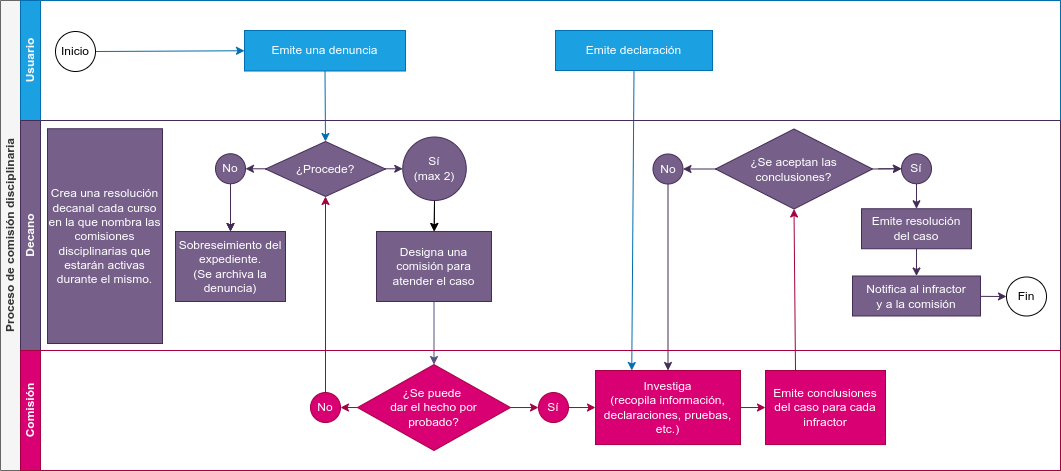
\includegraphics[width=1\textwidth]{images/process.png}
	\caption{Diagrama de carriles de piscina que modela el \proceso de \lafac}
	\label{fig:entities}
\end{figure}


\section[Conceptos]{Principales conceptos asociados al proceso de Comisi�n Disciplinaria en la Facultad 4}\label{concepts}

\newcommand{\ectx}{En el contexto del proceso de comisi�n disciplinaria se refiere}
\comment[carlosepc]{Buscar y citar las fuentes faltantes de las explicaciones de los conceptos.}
\paragraph{Denuncia:} Es la acci�n y efecto de denunciar (avisar, noticiar, declarar la irregularidad o ilegalidad de algo, delatar). La denuncia puede realizarse ante las autoridades correspondientes (lo que implica la puesta en marcha de un mecanismo judicial) o de forma p�blica (s�lo con valor testimonial) \citep{rae}. \ectx al documento emitido por un trabajador de la \uci en el que describe una indisciplina cometida por uno o varios estudiantes; con el objetivo de que se ponga en mar
\paragraph{Comisi�n disciplinaria:} Conjunto de personas encargadas por una autoridad de velar por la buena conducta y disciplina \citep{rae}. En el contexto del proceso analizado en este trabajo se refiere al equipo conformado por un jefe y un secretario, ambos profesores, que se encarga de la resoluci�n de un caso disciplinario. Si la indisciplina asociada al caso fue realizada en la residencia, pasan a formar parte de la comisi�n disciplinaria el representante de la residencia, quien es un trabajador de la misma, y un representante del edificio donde vive el estudiante.

\paragraph{Caso disciplinario:} Se crea cuando se aprueba una denuncia y se asigna una comisi�n disciplinaria para su an�lisis.

\paragraph{Expediente:} Instrumento administrativo que recopila la documentaci�n imprescindible que sustenta un acto administrativo \citep{rae}. En el contexto del proceso de comisi�n disciplinaria se refiere a resumen de la documentaci�n generada por un caso disciplinario.

\paragraph{Gesti�n:} Del lat�n gest\u{i}o, el concepto de gesti�n hace referencia a la acci�n y a la consecuencia de administrar o gestionar algo. Al respecto, hay que decir que gestionar es llevar a cabo diligencias que hacen posible la realizaci�n de una operaci�n comercial o de un anhelo cualquiera \citep{definicionde}.

\paragraph{Sistema de gesti�n:} Un sistema de gesti�n es una herramienta que permite controlar, planificar, organizar y automatizar las tareas administrativas de una organizaci�n. \citep{sistemadegestion}%todo

\paragraph{\ac{dms}:} Son todos aquellos creados para la gesti�n de grandes cantidades de documentos. Suelen rastrear, almacenar, archivar y organizar documentos electr�nicos o im�genes de documentos en papel. \citep{sistemadegestion} 

\paragraph{Servidor web:} Un servidor web o Servidor HTTP es una pieza de software de comunicaciones que intermedia entre el servidor en el que est�n alojados los datos solicitados y el computador del cliente, permitiendo conexiones bidireccionales o unidireccionales, s�ncronas o as�ncronas, con cualquier aplicaci�n del cliente, incluso con los navegadores que traducen un c�digo (renderizable) a una p�gina web determinada. O sea, se trata de programas que median entre el usuario de Internet y el servidor en donde est� la informaci�n que solicita \citep{yeager1996web}.

\paragraph{Aplicaci�n cliente:} Una aplicaci�n cliente es un paquete de software que funciona sobre el propio sistema operativo de un dispositivo (que puede ser por ejemplo un smartphone, una laptop o un equipo de escritorio). Es decir, que la aplicaci�n se instala y corre �dentro� del computador, o lo que solemos llamar tambi�n �de forma local�. En un computador, estas aplicaciones se instalan en el disco duro, donde guardan toda la informaci�n \citep{yeager1996web}. 

\paragraph{Aplicaci�n web:} En la ingenier�a de software se denomina aplicaci�n web (al igual se le denomina como "Software Web") a aquella herramienta que los usuarios pueden utilizar accediendo a un servidor web a trav�s de internet o una intranet mediante un navegador. En otras palabras, es un programa que se codifica en un lenguaje interpretable por los navegadores web en la que se conf�a, a estos, la ejecuci�n \citep{whatisawebapp}.
\section{Estudio del arte}
En esta secci�n se analizan soluciones inform�ticas existentes en Cuba y el mundo para problem�ticas similares.

\subsection{Sistemas en el �mbito internacional}
\subsubsection{Sistema de Control de Asistencia de Personal de IBIX}
El Sistema de Control de Asistencia de Personal de IBIX es un software que te permite llevar registro autom�tico del tiempo laborado e incidencias del personal en base a los turnos y pol�ticas definidas por la empresa. \citep{ibix_reporte_2013}
\paragraph{Caracter�sticas de inter�s}
\begin{description}
	\item[Reportes sencillos de analizar con informaci�n
	completa y exacta] Opci�n de generar un gran n�mero de reportes con los que cuenta el sistema, como los son los reportes de checadas, asistencias, ausentismos, retardos, tiempo extra, pre-n�mina, comedor y control de acceso.
	\item[Reportes din�micos a Excel] El sistema permite dise�ar y guardar plantillas de reportes en Excel con los datos de trabajadores que se deseen, teniendo disponibles todos los Datos de los trabajadores, la informaci�n de los turnos de la semana, la primer y ultima checada del d�a, as� como datos de la pre-n�mina

	\item[Configuraci�n de Usuarios] El sistema permite configurar las opciones a las que el usuario tiene acceso de esta forma definir las tareas que puede realizar un usuario en espec�fico; las empresas, celdas y departamentos a las que tiene permitido acceder.
\end{description}


El Sistema de Control de Asistencia de Personal verifica el registro de checadas y horarios del turno definido del trabajador, realizando un c�lculo preciso del tiempo laborado, tiempo extra, tiempo de labor en d�a de descanso, tiempo de labor en d�a festivo, adem�s de otros conceptos de incidencias.
Este sistema obliga el cumplimiento de la jornada de trabajo del personal y establece un control
sobre el tiempo extra, el cual representa un alto costo en las empresas. Mejora el desempe�o en el
registro de los trabajadores y productividad del personal. Es f�cil de usar en ambiente Windows XP,
7 ,8 y en sistemas multiusuario y multiempresa.

\paragraph{Dumbo: Portal Integrado para la Gesti�n de Peticiones de Cambio e Incidencias de la Universidad de Murcia}
Herramienta que integra de una manera �gil la gesti�n de incidencias y atenci�n a usuarios en las dos vertientes que �stas conllevan: los usuarios que las originan y los expertos que se encargan de resolverlas. Dumbo es considerado una Soluci�n tecnol�gicamente avanzada, atendiendo a que es un sistema web apoyado sobre una arquitectura de tres capas que garantiza f�cil acceso, instalaci�n cero e independencia de la plataforma cliente utilizada. Ofrece valiosa informaci�n a responsables de Sistemas de Informaci�n y a equipos directivos.\citep{acanda2018cdis}
Este sistema es privativo y ajustado a las necesidades propias del cliente. El mismo no es multiplataforma, solo opera en el sistema Windows, sin embargo, gestiona varios procesos de los cuales se pueden tomar ideas a la hora de definir los requisitos como son:
\begin{itemize}
	\item Solicitud de nuevas incidencias
	\item Exploraci�n de incidencias solicitadas
	\item Atenci�n de incidencias recibidas
	\item Gesti�n de la cola gen�rica de incidencias
	\item Administraci�n del sistema
	\item Alertas
	\item Notificaciones
\end{itemize}

\subsection{Sistemas en el �mbito nacional}
\begin{description}
	\item[\ac{cdis-2}] La Facultad 2 de la \uci posee un sistema inform�tico para la gesti�n de la informaci�n de expedientes disciplinarios en su versi�n 1.0. Dicha herramienta cuenta con la mayor�a de los procesos que se llevan actualmente a cabo por las comisiones disciplinarias, pero no todos est�n finalmente concluidos. En consecuencia	\ac{cdis-2} no permite emitir un reporte a la comisi�n sobre la cantidad de d�as h�biles que disponen antes de cerrar un expediente. En este sentido, la aplicaci�n existente no permite mostrarle, al asesor el estado de un expediente, la comisi�n que lo atiende ni si fue prorrogado por alguna causa. No permite realizar b�squedas dentro del sistema para conocer la cantidad de denuncias que existen o saber qu� comisi�n atiende a una denuncia determinada. Por otra parte, no es capaz de establecer opiniones entre los profesores, profesor gu�a, y otras personas involucradas en el proceso disciplinario; adem�s, no permite que en tiempo real pueda contar los d�as h�biles que poseen los expedientes en tr�mites.
		%No se ha puesto en explotaci�n por inconformidades t�cnicas del software.
		A�n no est� en explotaci�n ya que no cumple con los requisitos previstos por el cliente \citep{acanda2018cdis}.
	\item[\ac{codis}] Sistema que realiza el an�lisis y permite gestionar el proceso asociado a la Comisi�n Disciplinaria en la Facultad 3 de la \uci de forma eficiente, garantizando que se encuentre disponible la informaci�n completa de cada uno de los casos, las operaciones de adicionar denuncia, adicionar caso a una comisi�n, adicionar miembro a comisi�n, entre otras. Como resultado del mismo se obtiene un sistema funcional, que cumple con las necesidades que presenta la Facultad 3, lo que permite mejorar el funcionamiento de las Comisiones Disciplinarias
		%TODO
		\citep{fernandez_castillo_codis_2012}.
		%	\item[SGPCD]
	\item[Sistema inform�tico para el an�lisis de las indisciplinas de los estudiantes de la Facultad 4 (AIE Fac 4)] Este sistema dise�ado y desarrollado en 2015 como trabajo de diploma para optar por el t�tulo de Ingeniero en Ciencias Inform�ticas por el entonces estudiante de Ingenier�a en Ciencias Inform�ticas Gabriel Betancourt Carrasco bajo la tutor�a de la Dra. C. Dunia Mar�a Colom� Cede�o, no se encuentra en en explotaci�n en la actualidad. %por //TODO
		Dicho sitema no cuenta con las funcionalidades que satisfacen necesidades de informatizaci�n del proceso de comisi�n disciplinaria en \lafac en la actualidad actuales de la Facultad durante el
\end{description}
% Please add the following required packages to your document preamble:
% \usepackage{graphicx}
\begin{table}[]
    \centering
    \caption{Comparaci�n entre los sistemas hom�logos analizados}
    \resizebox{\textwidth}{!}{%
    \begin{tabular}{|l|l|l|l|l|l|}
    \hline
    \textbf{Sistema} & \textbf{\begin{tabular}[c]{@{}l@{}}Gesti�n de proceso de\\ comisi�n disciplinaria\end{tabular}} & \textbf{Multiplataforma} & \textbf{\begin{tabular}[c]{@{}l@{}}Generaci�n de\\ documentos\end{tabular}} & \textbf{Licencia} & Estado        \\ \hline
    DUMBO            & No                                                                                              & No                       & S�                                                                          & Privativo         & No disponible \\ \hline
    CA-IBIX          & No                                                                                              & No                       & S�                                                                          & Privativo         & No disponible \\ \hline
    CODIS            & S�                                                                                              & No                       & No                                                                          & Libre             & Descontinuado \\ \hline
    SIPCD            & S�                                                                                              & No                       & S�                                                                          & Libre             & Descontinuado \\ \hline
    AIE Fac 4        & S�                                                                                              & S�                       & No                                                                          & Libre             & Descontinuado \\ \hline
    CDis             & S�                                                                                              & S�                       & S�                                                                          & Libre             & Actualizado   \\ \hline
    \end{tabular}%
    }
\end{table}
\subsection{Conclusiones del estudio del arte}
Tras realizar el estudio de hom�logos se encuentra una ausencia de alternativas ya implementadas o dise�adas que permitan resolver la problem�tica planteada. Algunos de los softwares analizados sirvieron para tomar en cuenta sus implementaciones de usabilidad o dise�o de flujo de informaci�n, pero informatizan un proceso diferente al descrito. Otros, a pesar de informatizar procesos muy similares, fueron desarrollados a medida para funcionar en entornos con, aunque pocas, no superfluas diferencias, o bien no cuentan con funcionalidades que satisfagan los requerimientos actuales para la informatizaci�n del proceso de comisi�n disciplinaria en \lafac.

\section{Herramientas y tecnolog�as a utilizar}

Para el desarrollo de cualquier aplicaci�n, es necesario utilizar diferentes t�cnicas como: los patrones de dise�o o las metodolog�as de desarrollo de software, adem�s del uso de distintas herramientas como los compiladores o editores de c�digos. Aunque a simple vista parezca que la selecci�n de las tecnolog�as para desarrollar aplicaciones es f�cil, es totalmente lo contrario; para su correcta selecci�n, es necesario ver el problema a resolver desde diferentes �ngulos y posibles situaciones futuras. El presente ep�grafe aborda alguna de las diferentes herramientas que dan soluci�n a la problem�tica planteada.

\subsection{Patrones de dise�o: }

Seg�n el libro Dive Into Design Patterns, los patrones de dise�o son:
\begin{quote}
	``Soluciones t�picas a problemas comunes en el desarrollo de software. Se podr�a decir que son como planos predefinidos que pueden ser adaptados para resolver problemas en el dise�o de la codificaci�n de un programa~\citep{Shevts2019}.''
\end{quote}

Normalmente se confunden con algoritmos, porque ambos conceptos describen soluciones t�picas a problemas conocidos, mientras que un algoritmo describe una serie de pasos a seguir para lograr un objetivo, un patr�n es una descripci�n de alto nivel de la soluci�n, o sea, la codificaci�n de un mismo patr�n puede ser diferente en programas distintos~\citep{Shevts2019}.

Los patrones de dise�o difieren entre ellos debido a su complejidad, el nivel de detalles necesarios y la escala del sistema que se va a implementar. Los patrones de bajo nivel son llamados idiomas y usualmente solo se aplican a un lenguaje de programaci�n. Mientras que los patrones m�s universales y de m�s alto nivel, son llamados patrones arquitect�nicos. Estos �ltimos pueden ser usados en cualquier programa independiente del lenguaje en que sea programado y adem�s pueden ser utilizados para crear la arquitectura completa de un software~\citep{Shevts2019}. 

\subsubsection{Surgimiento de los patrones:}

En un principio, no fueron llamados patrones, ni estaban agrupados, sino que fueron soluciones que se repitieron una y otra vez en el desarrollo de software. Debido a esto, Erich Gamma, Jhon Vlissides, Ralph Johnson y Richard Helm en 1995 escribieron el libro ``Design Patterns: Elements of Reusable Object-Oriented software'', libro que reun�a y clasificaba las soluciones hasta ahora utilizadas. 

El concepto de patr�n se di� a conocer en el libro ``Pattern Language: Towns, Buildings, Construction'' del autor Christopher Alexander, donde se describ�a un lenguaje natural para la construcci�n de edificios. Teniendo el libro anteriormente mencionado como base, fue que estas soluciones a problemas repetitivos fueron nombradas como patrones de dise�o de programaci�n.

Con el tiempo, estas cuatro personas pasaron a llamarse Gang of Four (Banda de los cuatro) y a su vez el nombre del libro paso a ser ``The GOF book''.

\subsubsection{Tipos de patrones}
En total el libro recoge 23 patrones, divididos en tres categor�as seg�n su intenci�n:
\begin{itemize}
	\item Patrones Creacionales:
	\begin{itemize}
		\item Provee mecanismos para la creaci�n de objetos lo que incrementa la flexibilidad y la reutilizaci�n de c�digo existente.
	\end{itemize}
	\item Patrones Estructurales:
	\begin{itemize}
		\item Explica como ensamblar objetos y clases dentro de largas estructuras, mientras que la estructura se mantiene flexible y eficiente.
	\end{itemize}
	\item Patrones de Comportamiento:
	\begin{itemize}
		\item Se encarga de la comunicaci�n eficiente y la asignaci�n de responsabilidades entre los objetos.
	\end{itemize}
\end{itemize}

\subsection{Metodolog�as para el desarrollo de software:}

``Los softwares han sido parte de la vida cotidiana de la humanidad desde hace muchos a�os, pero su desarrollo comenz� de una manera muy desorganizada, ya que se basaba en actividades de codificar y arreglar los errores. Los softwares en su mayor�a eran creados sin seguir una l�nea de actividades, por lo que la estructura de estos pod�a variar frecuentemente. Pero como todo en la vida, llega un momento en que hay que organizar la forma en que se hacen las cosas, por lo que surgi� una alternativa llamada metodolog�a. Esta dictaba un proceso bien estructurado para la creaci�n de software, lo cual hac�a el desarrollo de estos m�s predictibles y eficientes''~\citep{Awad2005}.

Primero surgieron las metodolog�as tradicionales poseedoras un plan de trabajo extenso, debido a la documentaci�n de los requerimientos del software, seguidos por la especificaci�n de la arquitectura y una representaci�n de alto nivel del software a desarrollar. Debido a la cantidad de trabajo a realizar, las metodolog�as tradicionales pasaron a ser conocidas como metodolog�as pesadas. Mayormente se utilizaban en software con un alto impacto, ya sea para la vida o la sociedad. Pero los proyectos que no pose�an un impacto tan notable, tambi�n deb�an utilizar las metodolog�as pesadas, por lo que el trabajo era muy lento y lleno de dificultades~\citep{Awad2005}.

En respuesta al trabajo excesivo y minucioso en proyectos sin grandes repercusiones en la sociedad, nacieron las metodolog�as �giles, que fueron destinadas al desarrollo de software mediante la interacci�n con el cliente. Cambios en la estructura del proyecto de forma m�s seguida y un desarrollo r�pido, eran las caracter�sticas que m�s difer�an del prop�sito principal de las metodolog�as pesadas.


La siguiente tabla explica de forma resumida las diferencias que existen entre las metodolog�as �giles y las pesadas:

\begin{table}[h]\caption{Comparaci�n, Metodolog�as �giles VS Metodolog�as Tradicionales o Pesadas \citep{Awad2005}}
	\label{table:metodologies-comparison}
	\centering
	\begin{tabular}{|l|l|l|}
		\hline
		\theader
		\textbf{ Aspectos } 	& \textbf{Metodolog�as �giles}   & \textbf{ Metodolog�as Pesadas} \\ \hline
		Acercamiento dfsdf efwe			& Adaptivo 				  & Predictivo 				\\ \hline
		\stripe
		Medici�n del objetivo   & Valor para el negocio   & Conformaci�n del plan	\\ \hline
		Tama�o del proyecto		& Peque�o 				  & Largo 					\\ \hline
		\stripe
		Tipo de administraci�n  & Descentralizado 		  & Autocr�tico 			\\ \hline
		Perspectiva de cambios  & Adaptable a cambio 	  & Sostenible al cambio 	\\ \hline
		\stripe
		Cultura del equipo      & Liderazgo\textbackslash Colaboraci�n & Comandada\textbackslash Controlada \\ \hline
		Documentaci�n		    & Baja 					  & Pesada 					\\ \hline
		\stripe
		Orientada a 		    & Personas 				  & Procesos 				\\ \hline
		Ciclos de desarrollo    & Numerosos 			  & Limitados 				\\ \hline
		\stripe 
		Dominio de desarrollo   & Impredecibles 		  & Predecibles 			\\ \hline
		Planificaci�n inicial   & M�nima   				  & Comprensiva 			\\ \hline
		\stripe 
		Retorno de la inversi�n & Temprano en el proyecto & Al final del proyecto 	\\ \hline
		Tama�o del equipo 		& Peque�o 				  & Grande 					\\ \hline
		
	\end{tabular}
	
\end{table}

Como se vio anteriormente las metodolog�as se dividen en dos tipos, las metodolog�as �giles y las tradicionales, dentro de las �ltimas podemos encontrar:
\begin{itemize}
	\item Waterfall:
	\begin{itemize}
		\item En espa�ol Cascada.
		\item Hace �nfasis en una estructura progresiva entre diferentes fases del desarrollo del software. Cada fase contiene un conjunto de actividades definidas, por lo que deben ser cumplidas antes de pasar a la siguiente fase.
	\end{itemize}
	\item \ac{RUP}:
	\begin{itemize}
		\item Tambi�n conocida como Proceso Unificado de Rational.
		\item Organiza el desarrollo en flujo de trabajos y son realizados de forma iterativa e incremental.
	\end{itemize}
\end{itemize}

Dentro de las metodolog�as �giles est�n:
\begin{itemize}
	\item \ac{XP}
	\begin{itemize}
		\item Programaci�n Extrema.
		\item Se caracteriza por los ciclos de desarrollo cortos, el incremento de los planes para el desarrollo del software, adem�s de la retroalimentaci�n que se establece con el cliente.
	\end{itemize}
	\item SCRUM:
	\begin{itemize}
		\item Describe la forma en que los miembros de equipo deben trabajar para poder obtener un sistema flexible en un entorno que var�a de manera constante.
	\end{itemize}
	\item Agile Lite:
	\begin{itemize}
		\item ``(...)puede ser aplicada a cualquier proyecto, asumiendo que el trabajo a realizar se pueda dividir en peque�as acciones.''~\citep{AgileLiteHumanos}
		\item Utiliza ciclos de desarrollos cortos.
	\end{itemize}
\end{itemize}

Con la ayuda de la informaci�n anteriormente expuesta, ya es hora de seleccionar una metodolog�a para el desarrollo del \cdis, pero antes, se deben poner en una balanza las caracter�sticas del proyecto a desarrollar. El uso de la tabla anteriormente descrita \ref{tab:metodologias}, es de vital importancia para una correcta selecci�n de la metodolog�a a utlizar. Una vez balanceada, seg�n las necesidades requeridas para desarrollar el \cdis, esta ``gu�a'' toma la siguiente estructura:


% Please add the following required packages to your document preamble:
% \usepackage[table,xcdraw]{xcolor}
% If you use beamer only pass "xcolor=table" option, i.e. \documentclass[xcolor=table]{beamer}
\begin{table}[h]
	\centering
	\begin{tabular}{|l|l|l|}
		\hline
		\rowcolor[HTML]{C4BBD7} 
		{ } & { �giles} & { Pesadas} \\ \hline
		Acercamiento & X &  \\ \hline
		\stripe 
		Medici�n del objetivo & X &  \\ \hline
		Tama�o del proyecto & X &  \\ \hline
		\stripe 
		Tipo de administraci�n & X &  \\ \hline
		Perspectiva de cambios & X &  \\ \hline
		\stripe 
		Cultura del equipo & X &  \\ \hline
		Documentaci�n & X &  \\ \hline
		\stripe 
		Orientada & X &  \\ \hline
		Ciclos de desarrollo & X &  \\ \hline
		\stripe 
		Dominio de desarrollo &  & X \\ \hline
		Planificaci�n inicial & X &  \\ \hline
		\stripe 
		Retorno de la inversi�n &  & X \\ \hline
		Tama�o del equipo & X &  \\ \hline
		\stripe 
		Total: & 11 & 2 \\ \hline
	\end{tabular}
	\caption{Resultado de la selecci�n de la metodolog�a}
	\label{tab:resultado}
\end{table}

Seg�n la tabla anterior, el software debe ser desarrollado siguiendo las pautas de las metodolog�as �giles, ya que cumple 11 de los 13 par�metros necesarios para tomar la decisi�n.

Dentro de las posibles metodolog�as �giles a seleccionar se encuentras: \ac{XP}, Scrum, Agile Lite. Se decide utilizar \ac{XP}.

\subsubsection{Programaci�n Extrema:}

``Es una Metodolog�a ligera de desarrollo de aplicaciones que se basa en la simplicidad, la comunicaci�n y la realimentaci�n del c�digo desarrollado''~\citep{VALLADAREZ2016}.

Objetivos de \ac{XP}:
\begin{itemize}
	\item La satisfacci�n del cliente.
	\item Potenciar el trabajo en equipo.
	\item Minimizar el riesgo actuando sobre las variables del proyecto: costo, tiempo, calidad, alcance.
\end{itemize}

Caracter�sticas:
\begin{itemize}
	\item Metodolog�a basada en prueba y error para obtener un software que funcione correctamente.
	\item Es orientada hacia quien produce y usa el software.
	\item Reduce el costo de cambio en todas las etapas del ciclo de vida de la aplicaci�n.
	\item Cliente bien definido.
	\item Los requisitos pueden cambiar.
\end{itemize}

\textbf{Artefactos de la metodolog�a \ac{XP}:}

\textbf{Historia de usuarios:}

Las \ac{HU} representan una breve descripci�n del comportamiento del sistema. Se realizan por cada caracter�stica principal del sistema y son utilizadas para cumplir estimaciones de tiempo y el plan de lanzamientos, as� mismo reemplazan un gran documento de requisitos y presiden la creaci�n de las pruebas de aceptaci�n~\citep{VALLADAREZ2016}..

Cada \ac{HU} debe ser lo suficientemente comprensible y delimitada para que los programadores puedan implementarlas en unas semanas.



\textbf{Tareas de ingenier�a:}

Una \ac{HU} se descompone en varias tareas de ingenier�a, que describen las actividades que se realizar�n en cada \ac{HU}, as� mismo las tareas de ingenier�a se vinculan m�s al desarrollador, ya que permite tener un acercamiento con el c�digo~\citep{VALLADAREZ2016}.. 

%Esta puede ser vista en la tabla \ref{tab:ti}.
%
%\begin{table}[h]
%	\centering
%	\begin{tabular}{|l|l|}
%		\hline
%		\rowcolor[HTML]{C4BBD7} 
%		\multicolumn{2}{|c|}{\cellcolor[HTML]{C4BBD7}{Tarea de Ingenier�a}} \\ \hline
%		N�mero de tarea:  Identificador de la tarea. & \begin{tabular}[|c|]{@{}l@{}}  N�mero de historia: N�mero asignado \\ de la historia correspondiente. \end{tabular}\\ \hline
%		\stripe 
%		\multicolumn{2}{|l|}{\cellcolor[HTML]{EDEBF1}Nombre de Tarea: Describe de manera general dicha tarea.} \\ \hline
%		Tipo de tarea: Tipo al que corresponde dicha tarea. & \begin{tabular}[|c|]{@{}l@{}} Puntos estimados: N�meros de d�as necesarios \\ para desarrollar dicha tarea. \end{tabular} \\ \hline
%		\stripe 
%		Fecha Inicio: Fecha inicial de la creaci�n de dicha tarea. & Fecha Fin: Fecha de la culminaci�n de dicha tarea. \\ \hline
%		\multicolumn{2}{|l|}{Programador Responsable: Nombre del programador a cargo de desarrollar la tarea.} \\ \hline
%		\stripe 
%		\multicolumn{2}{|l|}{\cellcolor[HTML]{EDEBF1}Descripci�n: Informaci�n detallada de dicha tarea.} \\ \hline
%	\end{tabular}
%	\caption{Plantilla: Tarea de Ingenier�a.}
%	\label{tab:ti}
%\end{table}



\textbf{Pruebas de aceptaci�n:}

Antes de conocer en qu� consisten las pruebas de aceptaci�n, es necesario conocer los dos tipos de pruebas que  existen, hoy d�a, en la industria del software~\citep{Nidhra2012}:

\begin{itemize}
	\item \textbf{Caja negra}: Son las pruebas basadas en los requerimientos especificados y no es necesario examinar el c�digo.
	
	\item \textbf{Caja blanca}: Prueba aplicable �nicamente sobre el c�digo perteneciente a un software desarrollado. Son dise�ados desde el punto de vista del desarrollador. Es principalmente usado para detectar errores l�gicos en el c�digo de un programa. 
\end{itemize}

Las pruebas de aceptaci�n pertenecen a la categor�a de pruebas de caja negra y son de vital importancia para el �xito de una iteraci�n y el comienzo de la siguiente, con lo cual el cliente puede conocer el avance en el desarrollo del sistema y a los programadores lo que les resta por hacer. Adem�s, permite una retroalimentaci�n para el desarrollo de las pr�ximas historias de usuarios a ser entregadas. Estas son com�nmente llamadas pruebas del cliente, por lo que las realiza el encargado de verificar si las historias de usuarios de cada iteraci�n cumplen con la funcionalidad esperada~\citep{XPACT}. 
%
%Esta plantilla puede ser vista en la tabla \ref{tab:pa}.
%% Please add the following required packages to your document preamble:
%% \usepackage[table,xcdraw]{xcolor}
%% If you use beamer only pass "xcolor=table" option, i.e. \documentclass[xcolor=table]{beamer}
%\begin{table}[h]
%	\centering
%	\begin{tabular}{|l|l|}
%		\hline
%		\multicolumn{2}{|c|}{\cellcolor[HTML]{C4BBD7}Prueba de aceptaci�n} \\ \hline
%		\begin{tabular}[c]{@{}l@{}}C�digo: N� �nico, permite identificar \\ la prueba de aceptaci�n.\end{tabular} & \begin{tabular}[c]{@{}l@{}}N� Historia de Usuario: N�mero �nico \\ que identifica a la historia de usuario.\end{tabular} \\ \hline
%		\multicolumn{2}{|l|}{\cellcolor[HTML]{EDEBF1}\begin{tabular}[c]{@{}l@{}}Historia de Usuario: Nombre que indica de manera general \\ la descripci�n de la historia de usuario.\end{tabular}} \\ \hline
%		\multicolumn{2}{|l|}{\begin{tabular}[c]{@{}l@{}}Condiciones de Ejecuci�n: Condiciones previas que deben \\ cumplirse para realizar la prueba de aceptaci�n.\end{tabular}} \\ \hline
%		\multicolumn{2}{|l|}{\cellcolor[HTML]{EDEBF1}\begin{tabular}[c]{@{}l@{}}Entrada/Pasos de Ejecuci�n: Pasos que siguen los usuarios \\ para probar la funcionalidad de la historia de usuario.\end{tabular}} \\ \hline
%		\multicolumn{2}{|l|}{\begin{tabular}[c]{@{}l@{}}Resultado Esperado: Respuesta del sistema que el cliente espera, \\ despu�s de haber ejecutado una funcionalidad\end{tabular}} \\ \hline
%		\multicolumn{2}{|l|}{\cellcolor[HTML]{EDEBF1}\begin{tabular}[c]{@{}l@{}}Evaluaci�n de la Prueba: Nivel de satisfacci�n del cliente sobre \\ la respuesta del sistema. Los niveles son: Aprobada y No Aprobada.\end{tabular}} \\ \hline
%	\end{tabular}
%	\caption{Pruebas de aceptaci�n}
%	\label{tab:pa}
%\end{table}

\textbf{Tarjetas CRC (Clase \textbackslash Responsabilidades \textbackslash Colaboradores)}

Las Tarjetas \ac{CRC}, permiten conocer que clases componen el sistema y cuales interact�an entre s�.
%
%\begin{table}[h]
%	\centering
%	\begin{tabular}{|l|l|}
%		\multicolumn{2}{c}{\cellcolor[HTML]{C4BBD7}{Tarjeta CRC}} \\\hline
%		Nombre de la clase & \begin{tabular}[c]{@{}l@{}}N�mero de Historia: N�mero\\   de la historia de usuario correspondiente.\end{tabular} \\\hline
%		\multicolumn{2}{l}{\cellcolor[HTML]{EDEBF1}Responsabilidades: Atributos y operaciones de la clase.} \\ \hline
%	\end{tabular} 
%	\caption{Plantilla: Tarjeta CRC}
%	\label{tab:crc}
%\end{table}
\pagebreak

\textbf{Fases de la programaci�n \ac{XP}:}

\begin{figure}[h]
	\centering
	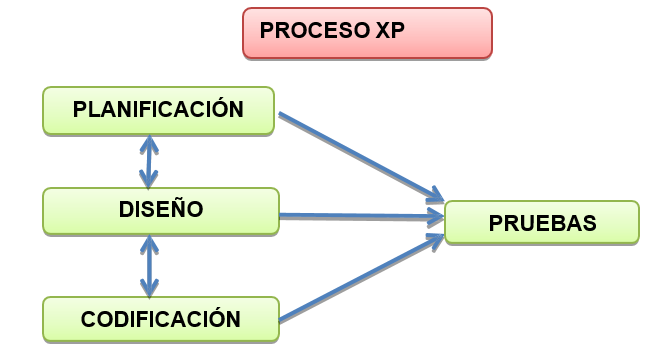
\includegraphics[width=.6\linewidth]{xp.png}
	\caption{Fases de XP ~\citep{VALLADAREZ2016}.}
	\label{fig:xp}
\end{figure}

\begin{itemize}
	\item \textbf{Planificaci�n}: La Metodolog�a \ac{XP} plantea la planificaci�n como un di�logo continuo entre las partes involucradas en el proyecto, incluyendo al cliente, a los programadores y a los coordinadores. El proyecto comienza recopilando las historias de usuarios, las que constituyen a los tradicionales casos de uso. Una vez obtenidas estas historias de usuarios, los programadores eval�an r�pidamente el tiempo de desarrollo de cada una, determinando as� el tiempo total de desarrollo del software.
	\item \textbf{Dise�o}: Especificaci�n de c�mo debe ser el dise�o final de la aplicaci�n, haciendo �nfasis en que un dise�o sencillo es m�s f�cil de implementar que uno complejo.
	\item \textbf{Codificaci�n}: Implementaci�n de los c�digos necesarios para satisfacer las historias de usuario.
	\item \textbf{Pruebas}: Una vez terminada la codificaci�n, se deben realizar las pruebas pertinentes a la misma.
\end{itemize}

\section*{Conclusiones del cap�tulo}
\begin{itemize}
    \item El estudio de los referentes te�ricos-metodol�gicos asociados a la gesti�n de procesos disciplinarios sirvi� de sustento al \cdis.
    \item El an�lisis de los sistemas hom�logos nacionales e internacionales permiti� definir aspectos importantes del dise�o e implementaci�n tales como artefactos ingenieriles de apoyo, tecnolog�as y herramientas; y de la investigaci�n como la documentaci�n a consultar.
    \item La selecci�n de la metodolog�a \ac{xp}, junto a las herramientas y tecnolog�as, definieron el ambiente de desarrollo que guiar� el desarrollo del \cdis.
\end{itemize}
%	PATRONES DE DISE�O
